\documentclass[a4paper]{article}
\usepackage[margin=1in]{geometry}
\linespread{1.2}
%\overfullrule=2cm % for debugging purposes! comment in production
% displays overfill rule on side of the document

\usepackage[utf8]{inputenc}
\usepackage[english,polish]{babel}

% babel defines \lll
\let\babellll\lll
\let\lll\relax

\usepackage[htt]{hyphenat}
\usepackage{amsmath}
\usepackage{amssymb}
\usepackage{amsthm}
\usepackage{blindtext}
\usepackage{enumerate}
\usepackage{enumitem}
\usepackage{graphicx}
\usepackage{mathtools}
\usepackage{multicol}
\usepackage{polski}
%\usepackage[T1]{fontenc}
%\usepackage[scaled]{beramono}
\usepackage{hyperref}

\usepackage{color}
\definecolor{bluekeywords}{rgb}{0.13,0.13,1}
\definecolor{greencomments}{rgb}{0,0.5,0}
\definecolor{redstrings}{rgb}{0.9,0,0}

\usepackage{listings}
\lstset{language=[Sharp]C,
	showspaces=false,
	showtabs=false,
	breaklines=false,
	showstringspaces=false,
	breakatwhitespace=true,
	escapeinside={(*@}{@*)},
	commentstyle=\color{greencomments},
	%keywordstyle=\color{bluekeywords}\bfseries,
	stringstyle=\color{redstrings},
	basicstyle=\ttfamily
}


\title{Wstęp do Algorytmów Ewolucyjnych \\
	\large Raport z testów}

\date{\today}
\author{Kacper Sarnacki \and Monika Żurkowska}

\begin{document}
\maketitle

\section{Przypomnienie}
Celem naszego projektu było zaimplementowanie zmodyfikowanego algorytmu ewolucji różnicowej, w którym jako pierwszy z 3 punktów stosowanych podczas mutacji wybierana była średnia punktów populacji a następnie porównanie tego rozwiązanie z klasycznym algorytmem ewolucji różnicowej wykorzystując benchmark ''cec2013'' do testowania.

\section{Lista zmian}
W związku z długim czasem wykonywania się testów zmuszeni byliśmy przyjąć kilka poprawek w stosunku do przyjętych założeń ze Specyfikacji Wstępnej:

\begin{itemize}
\item Rozmiar wektorów dla których przeprowadziliśmy testy: 5 oraz 10
\item Mniejsza liczba kombinacji współczynników F i Cr (patrz \ref{sec:testy})
\item Liczba iteracji dla każdego testu: 10
\item  Algorytm porównujemy wyłącznie z klasycznym algorytmem z losowym doborem 3 punktów w przeciwieństwie do wcześniejszego założenia o porównaniu go z algorytmem losowym i algorytmem, w którym jako pierwszy z trzech punktów wybierany jest najlepszy spośród obecnej populacji
\item W warunku stopu dla algorytmów brana była pod uwagę liczba wywołań funkcji ewaluacyjnej zamiast - jak wcześniej założono - liczby iteracji.
\end{itemize}

\section{Testy}
\label{sec:testy}
Zgodnie z wymaganiami, nasze testy przeprowadziliśmy na benchmarku ''cec2013' dla naszego algorytmu oraz dla algorytmu klasycznego. Wyniki przedstawione zostały w tabelach poniżej.
\newpage

\begin{figure}[!h]
\centering
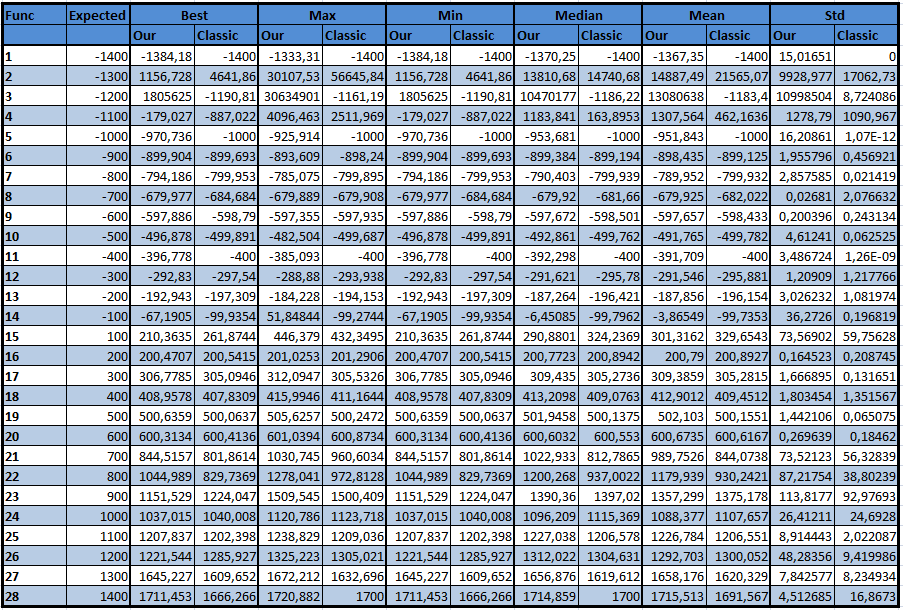
\includegraphics[width=\textwidth]{F25Cr25L5tab.png}
\caption{5-wymiarowa populacja. Wyniki dla parametrów: F = 0.25, Cr = 0.25}
\end{figure}

\begin{figure}[!h]
\centering
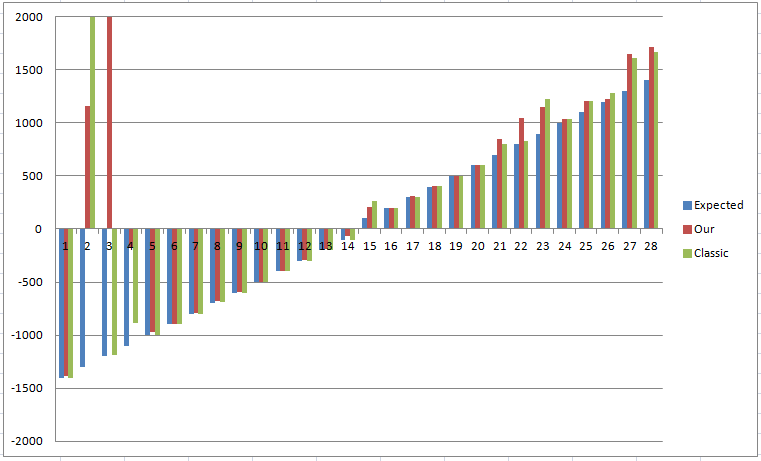
\includegraphics[width=\textwidth]{F25Cr25L5chart.png}
\caption{5-wymiarowa populacja. Wykres porównujący najlepsze rozwiązania dla naszego algorytmu oraz klasycznego. Parametry: F = 0.25, Cr = 0.25}
\end{figure}

\begin{figure}[!h]
\centering
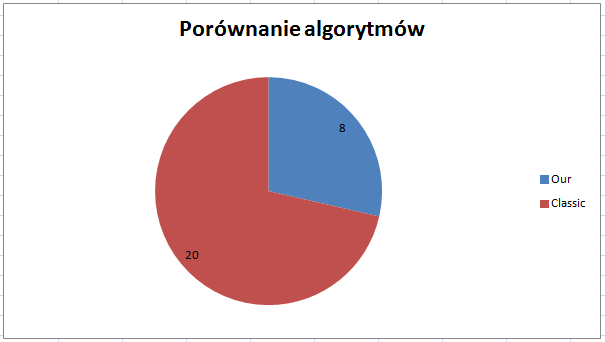
\includegraphics[width=\textwidth]{F25Cr25L5statystyka.png}
\caption{5-wymiarowa populacja. Parametry: F = 0.25, Cr = 0.25. Wykres porównujący liczbę lepiej znalezionych rozwiązań pomiędzy dwoma algorytmami.}
\end{figure}

\begin{figure}[!h]
\centering
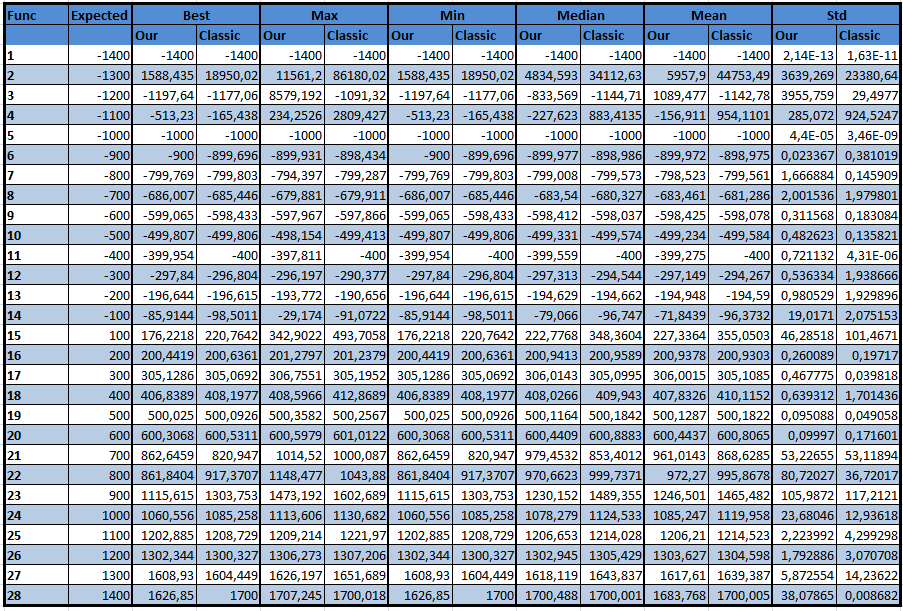
\includegraphics[width=\textwidth]{F5Cr25L5tab.png}
\caption{5-wymiarowa populacja. Wyniki dla parametrów: F = 0.5, Cr = 0.25}
\end{figure}

\begin{figure}[!h]
\centering
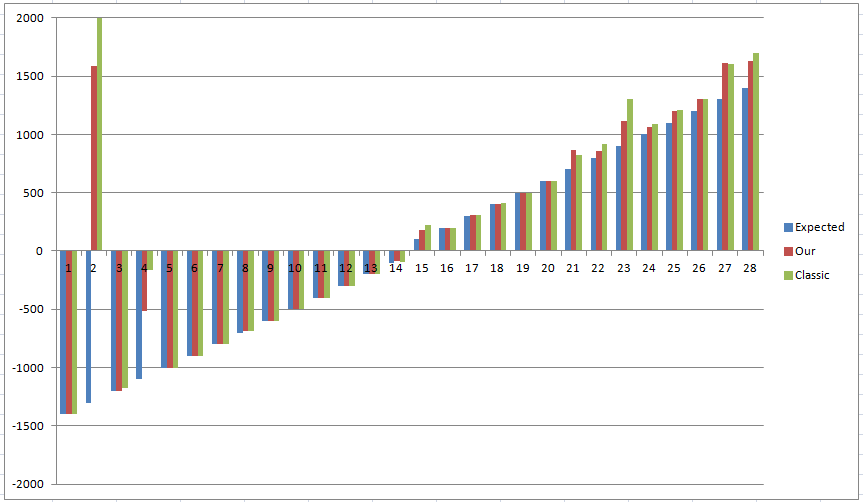
\includegraphics[width=\textwidth]{F5Cr25L5chart.png}
\caption{5-wymiarowa populacja. Wykres porównujący najlepsze rozwiązania dla naszego algorytmu oraz klasycznego. Parametry: F = 0.5, Cr = 0.25}
\end{figure}

\begin{figure}[!h]
\centering
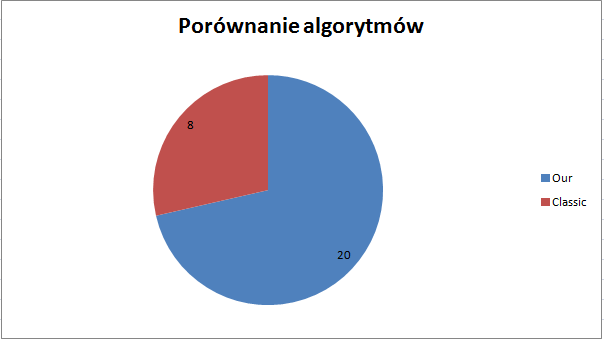
\includegraphics[width=\textwidth]{F5Cr25L5statystyka.png}
\caption{5-wymiarowa populacja. Parametry: F = 0.5, Cr = 0.25. Wykres porównujący liczbę lepiej znalezionych rozwiązań pomiędzy dwoma algorytmami.}
\end{figure}

\begin{figure}[!h]
\centering
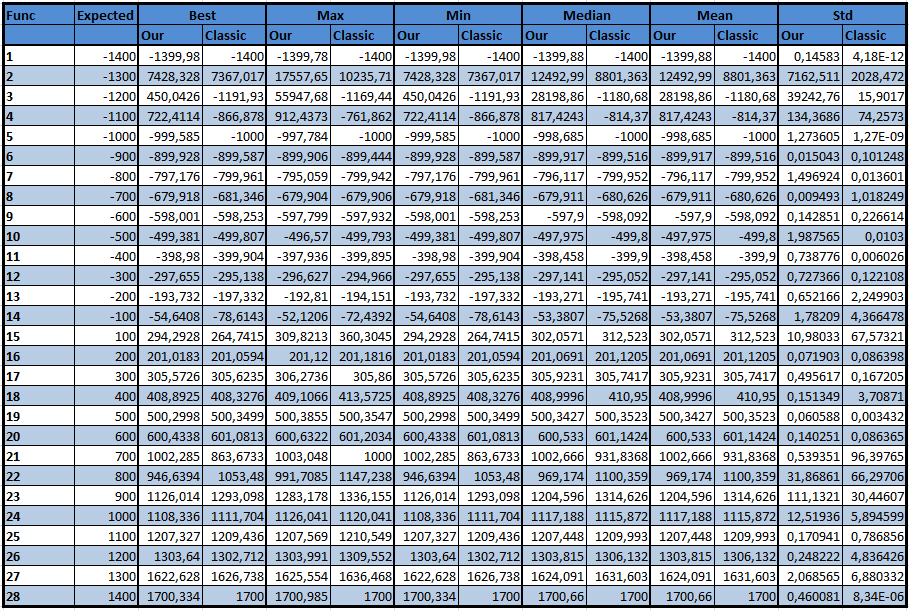
\includegraphics[width=\textwidth]{F5Cr5L5tab.png}
\caption{5-wymiarowa populacja. Wyniki dla parametrów: F = 0.5, Cr = 0.5}
\end{figure}

\begin{figure}[!h]
\centering
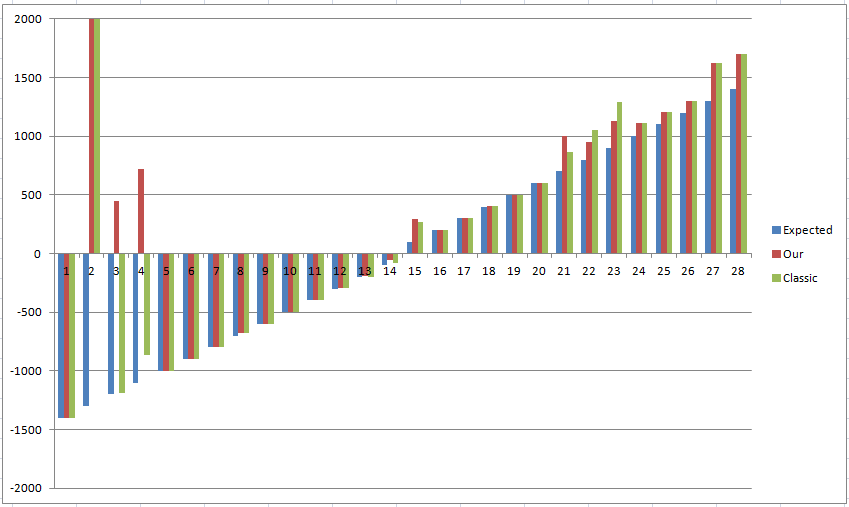
\includegraphics[width=\textwidth]{F5Cr5L5chart.png}
\caption{5-wymiarowa populacja. Wykres porównujący najlepsze rozwiązania dla naszego algorytmu oraz klasycznego. Parametry: F = 0.5, Cr = 0.5}
\end{figure}

\begin{figure}[!h]
\centering
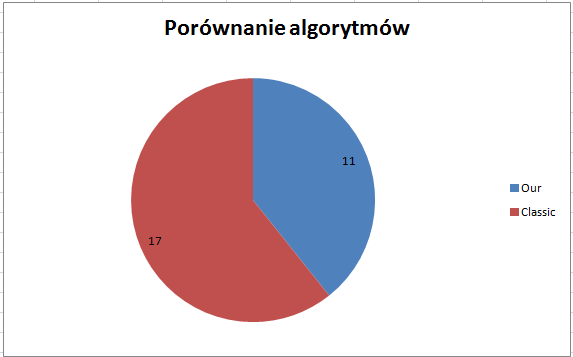
\includegraphics[width=\textwidth]{F5Cr5L5statystyka.png}
\caption{5-wymiarowa populacja. Parametry: F = 0.5, Cr = 0.5. Wykres porównujący liczbę lepiej znalezionych rozwiązań pomiędzy dwoma algorytmami.}
\end{figure}

\begin{figure}[!h]
\centering
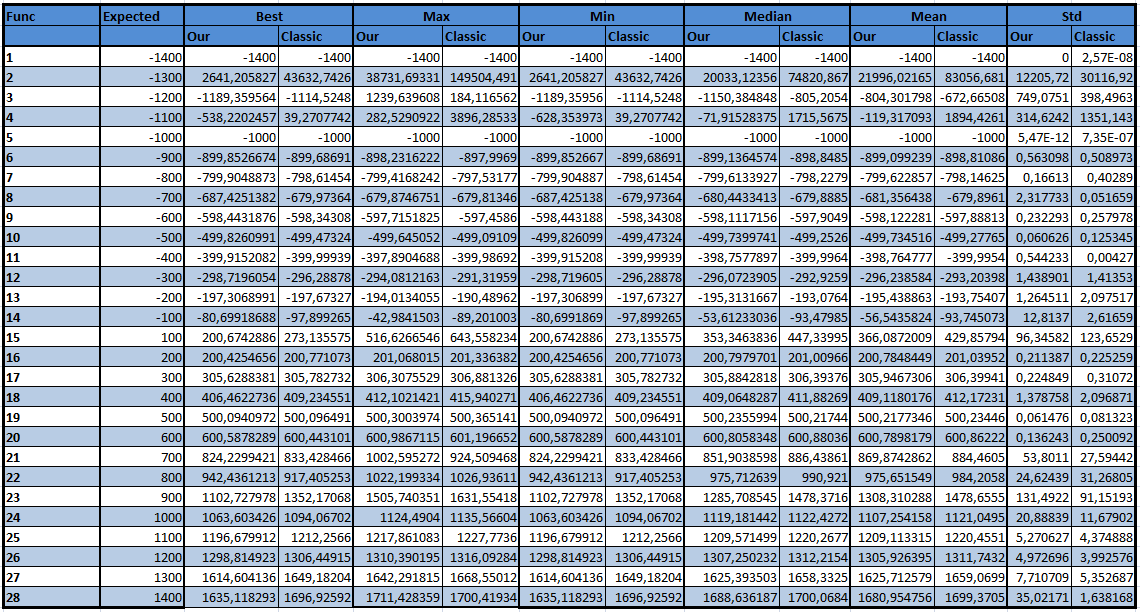
\includegraphics[width=\textwidth]{F75Cr25L5tab.png}
\caption{5-wymiarowa populacja. Wyniki dla parametrów: F = 0.75, Cr = 0.25}
\end{figure}

\begin{figure}[!h]
\centering
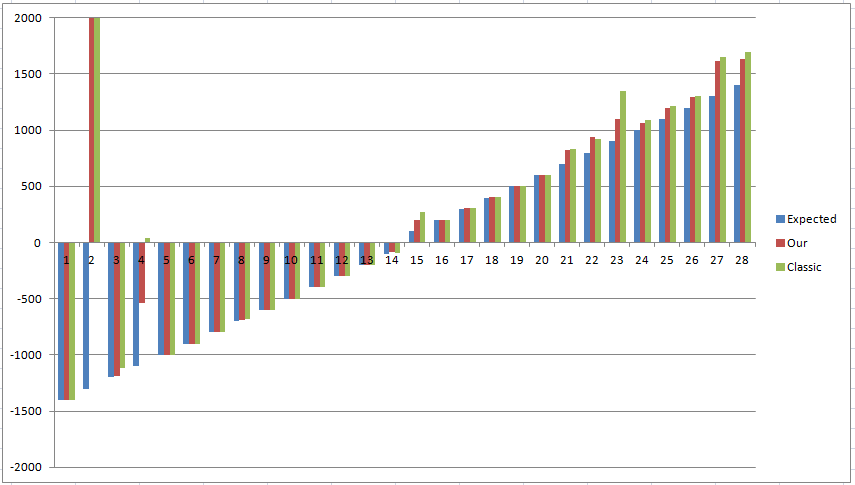
\includegraphics[width=\textwidth]{F75Cr25L5chart.png}
\caption{5-wymiarowa populacja. Wykres porównujący najlepsze rozwiązania dla naszego algorytmu oraz klasycznego. Parametry: F = 0.75, Cr = 0.25}
\end{figure}

\begin{figure}[!h]
\centering
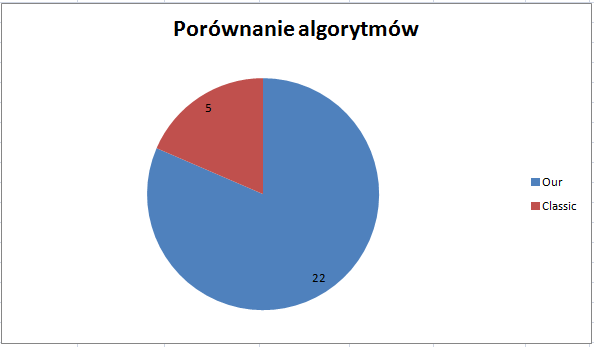
\includegraphics[width=\textwidth]{F75Cr25L5statystyka.png}
\caption{5-wymiarowa populacja. Parametry: F = 0.75, Cr = 0.25. Wykres porównujący liczbę lepiej znalezionych rozwiązań pomiędzy dwoma algorytmami.}
\end{figure}

\begin{figure}[!h]
\centering
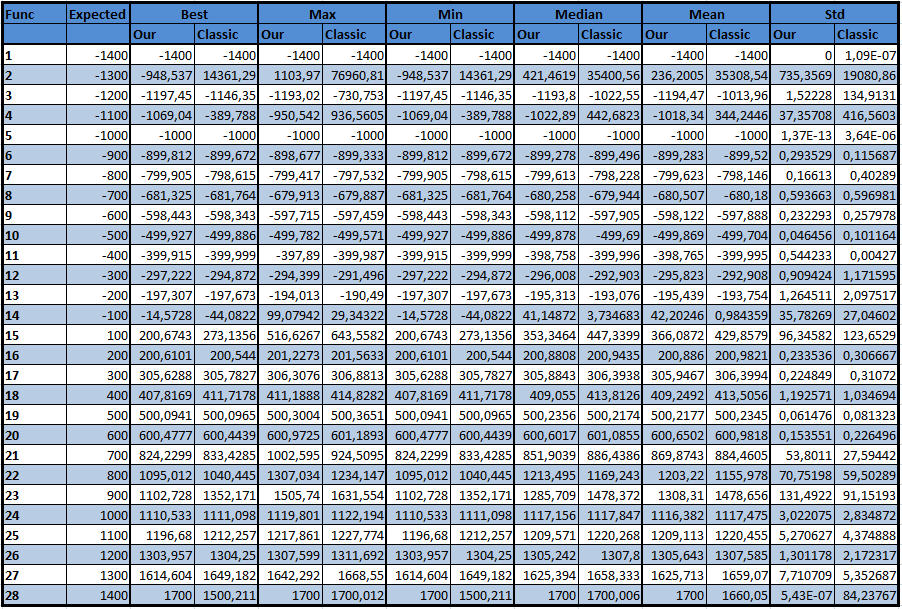
\includegraphics[width=\textwidth]{F75Cr5L5tab.png}
\caption{5-wymiarowa populacja. Wyniki dla parametrów: F = 0.75, Cr = 0.5}
\end{figure}

\begin{figure}[!h]
\centering
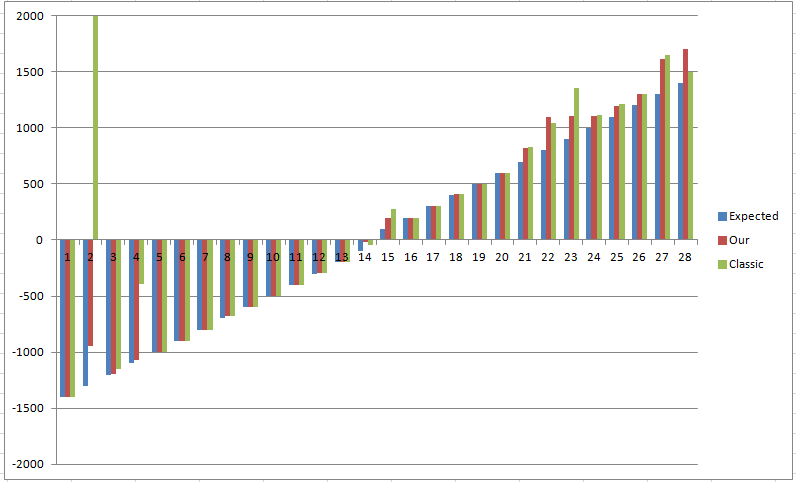
\includegraphics[width=\textwidth]{F75Cr5L5chart.png}
\caption{5-wymiarowa populacja. Wykres porównujący najlepsze rozwiązania dla naszego algorytmu oraz klasycznego. Parametry: F = 0.75, Cr = 0.5}
\end{figure}

\begin{figure}[!h]
\centering
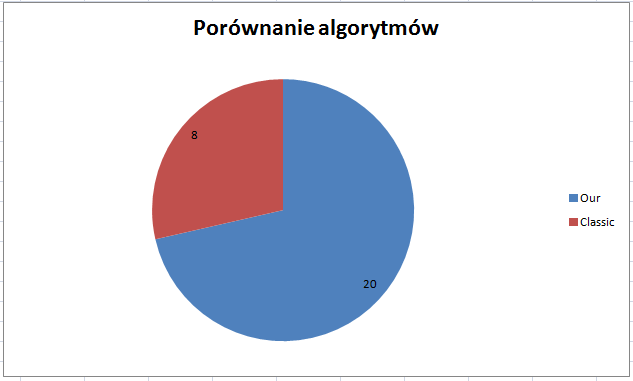
\includegraphics[width=\textwidth]{F75Cr5L5statystyka.png}
\caption{5-wymiarowa populacja. Parametry: F = 0.75, Cr = 0.5. Wykres porównujący liczbę lepiej znalezionych rozwiązań pomiędzy dwoma algorytmami.}
\end{figure}

\begin{figure}[!h]
\centering
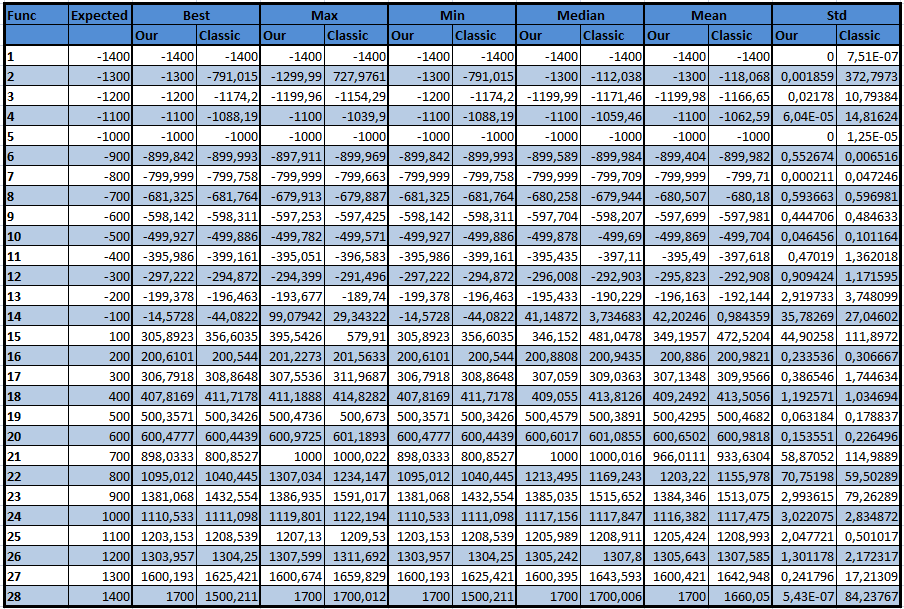
\includegraphics[width=\textwidth]{F75Cr75L5tab.png}
\caption{5-wymiarowa populacja. Wyniki dla parametrów: F = 0.75, Cr = 0.75}
\end{figure}

\begin{figure}[!h]
\centering
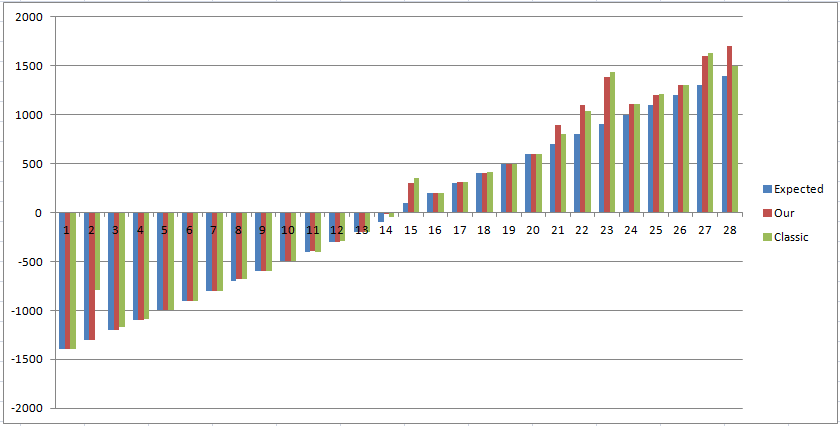
\includegraphics[width=\textwidth]{F75Cr75L5chart.png}
\caption{5-wymiarowa populacja. Wykres porównujący najlepsze rozwiązania dla naszego algorytmu oraz klasycznego. Parametry: F = 0.75, Cr = 0.75}
\end{figure}

\begin{figure}[!h]
\centering
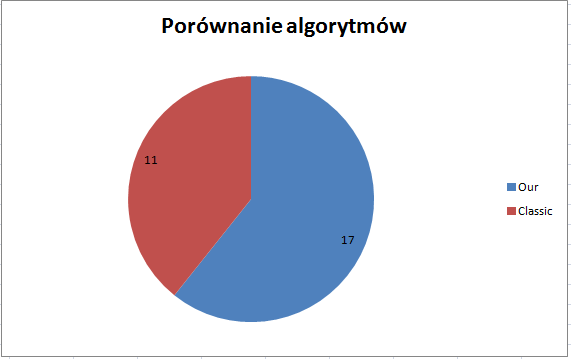
\includegraphics[width=\textwidth]{F75Cr75L5statystyka.png}
\caption{5-wymiarowa populacja. Parametry: F = 0.75, Cr = 0.75. Wykres porównujący liczbę lepiej znalezionych rozwiązań pomiędzy dwoma algorytmami.}
\end{figure}

\begin{figure}[!h]
\centering
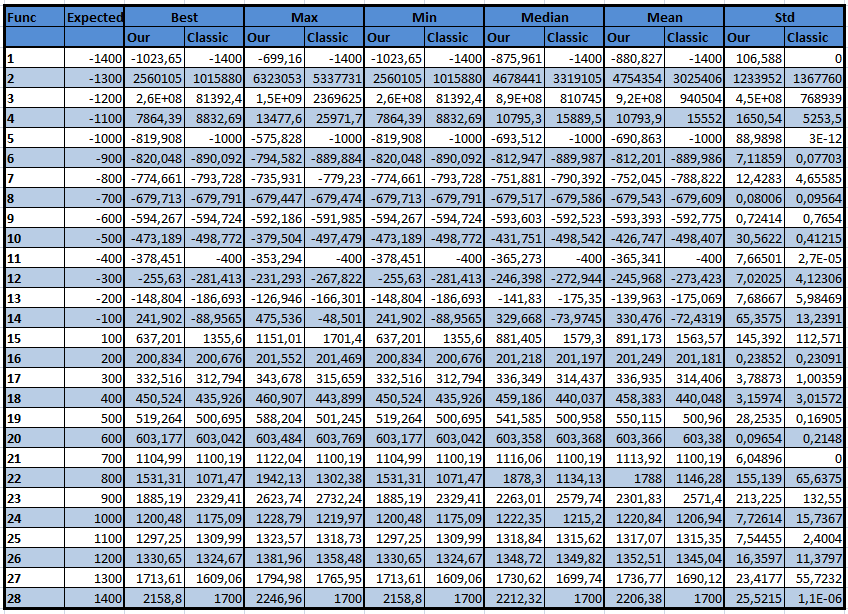
\includegraphics[width=\textwidth]{F25Cr25L10tab.png}
\caption{10-wymiarowa populacja. Wyniki dla parametrów: F = 0.25, Cr = 0.25}
\end{figure}

\begin{figure}[!h]
\centering
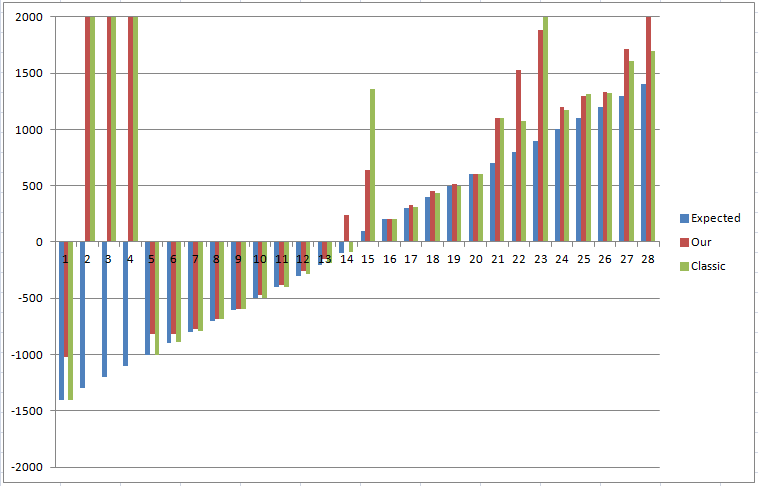
\includegraphics[width=\textwidth]{F25Cr25L10chart.png}
\caption{10-wymiarowa populacja. Wykres porównujący najlepsze rozwiązania dla naszego algorytmu oraz klasycznego. Parametry: F = 0.25, Cr = 0.25}
\end{figure}

\begin{figure}[!h]
\centering
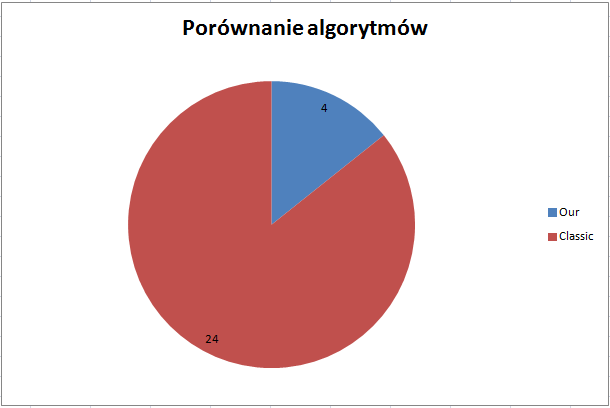
\includegraphics[width=\textwidth]{F25Cr25L10statystyka.png}
\caption{10-wymiarowa populacja. Parametry: F = 0.25, Cr = 0.25. Wykres porównujący liczbę lepiej znalezionych rozwiązań pomiędzy dwoma algorytmami.}
\end{figure}

\begin{figure}[!h]
\centering
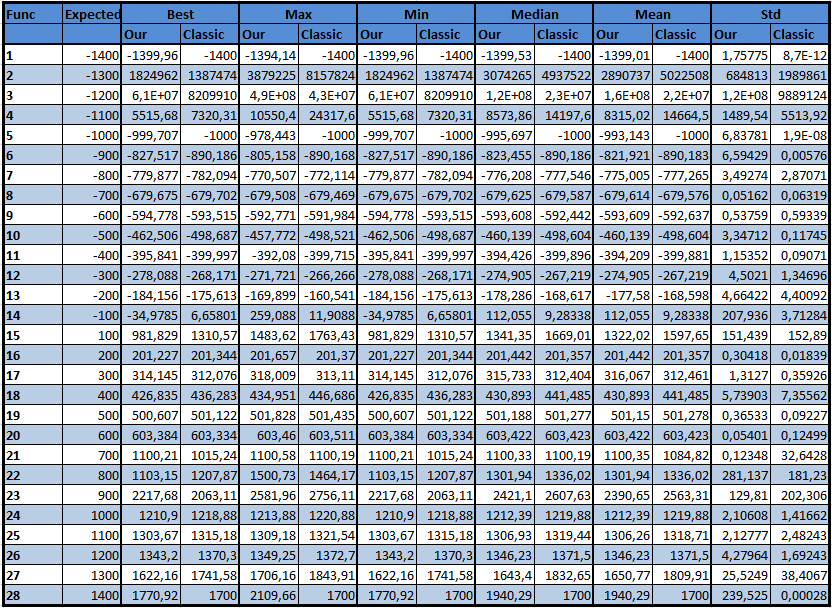
\includegraphics[width=\textwidth]{F5Cr25L10tab.png}
\caption{10-wymiarowa populacja. Wyniki dla parametrów: F = 0.5, Cr = 0.25}
\end{figure}

\begin{figure}[!h]
\centering
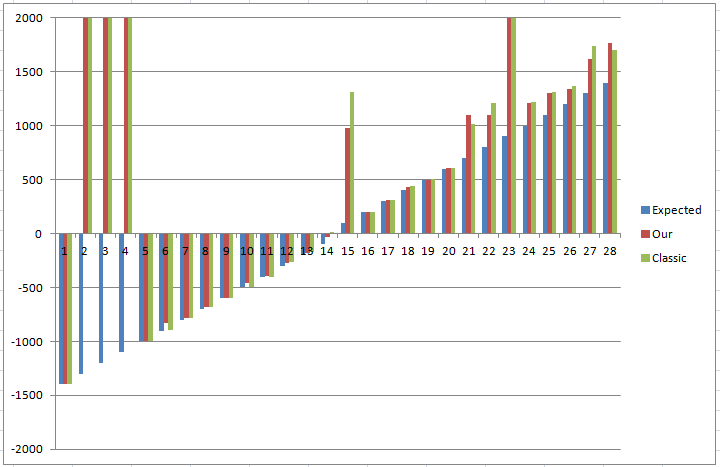
\includegraphics[width=\textwidth]{F5Cr25L10chart.png}
\caption{10-wymiarowa populacja. Wykres porównujący najlepsze rozwiązania dla naszego algorytmu oraz klasycznego. Parametry: F = 0.5, Cr = 0.25}
\end{figure}

\begin{figure}[!h]
\centering
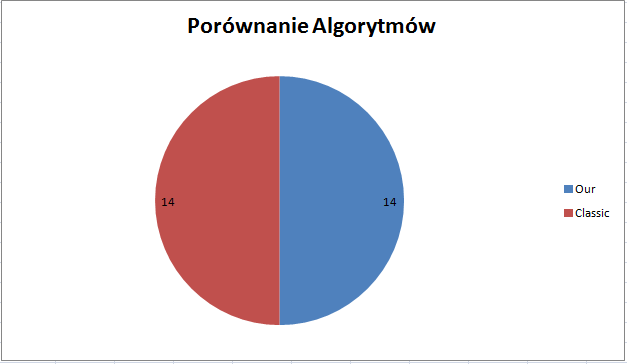
\includegraphics[width=\textwidth]{F5Cr25L10statystyka.png}
\caption{10-wymiarowa populacja. Parametry: F = 0.5, Cr = 0.25. Wykres porównujący liczbę lepiej znalezionych rozwiązań pomiędzy dwoma algorytmami.}
\end{figure}

\begin{figure}[!h]
\centering
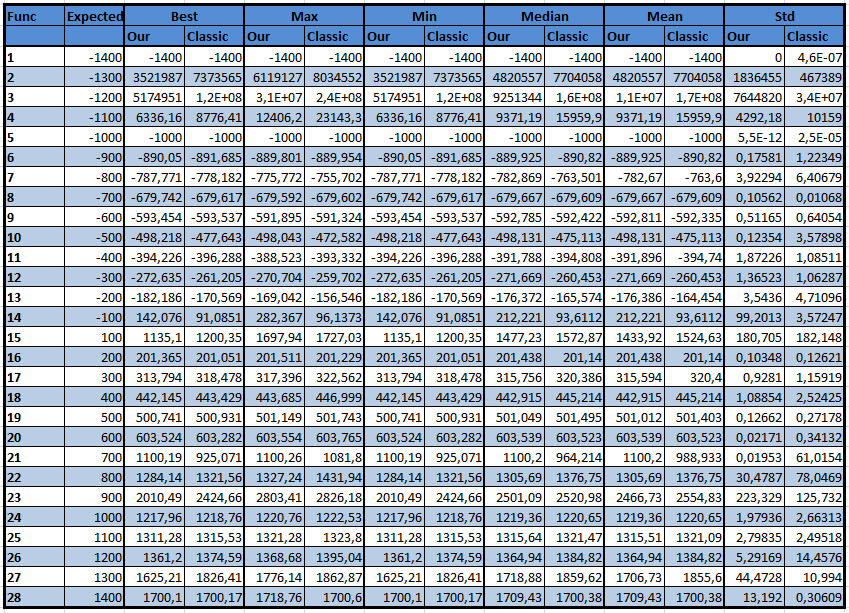
\includegraphics[width=\textwidth]{F75Cr25L10tab.png}
\caption{10-wymiarowa populacja. Wyniki dla parametrów: F = 0.75, Cr = 0.25}
\end{figure}

\begin{figure}[!h]
\centering
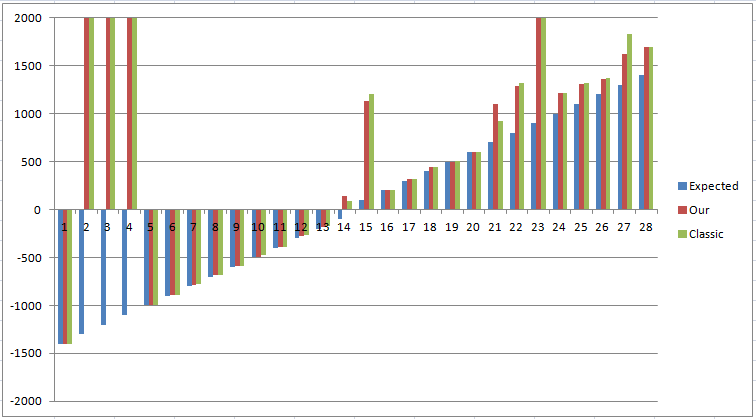
\includegraphics[width=\textwidth]{F75Cr25L10chart.png}
\caption{10-wymiarowa populacja. Wykres porównujący najlepsze rozwiązania dla naszego algorytmu oraz klasycznego. Parametry: F = 0.75, Cr = 0.25}
\end{figure}

\begin{figure}[!h]
\centering
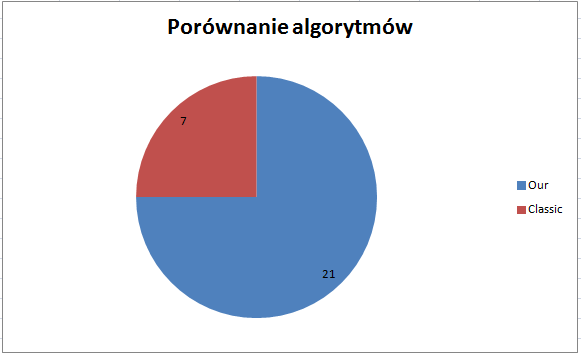
\includegraphics[width=\textwidth]{F75Cr25L10statystyka.png}
\caption{10-wymiarowa populacja. Parametry: F = 0.75, Cr = 0.25. Wykres porównujący liczbę lepiej znalezionych rozwiązań pomiędzy dwoma algorytmami.}
\end{figure}

\begin{figure}[!h]
\centering
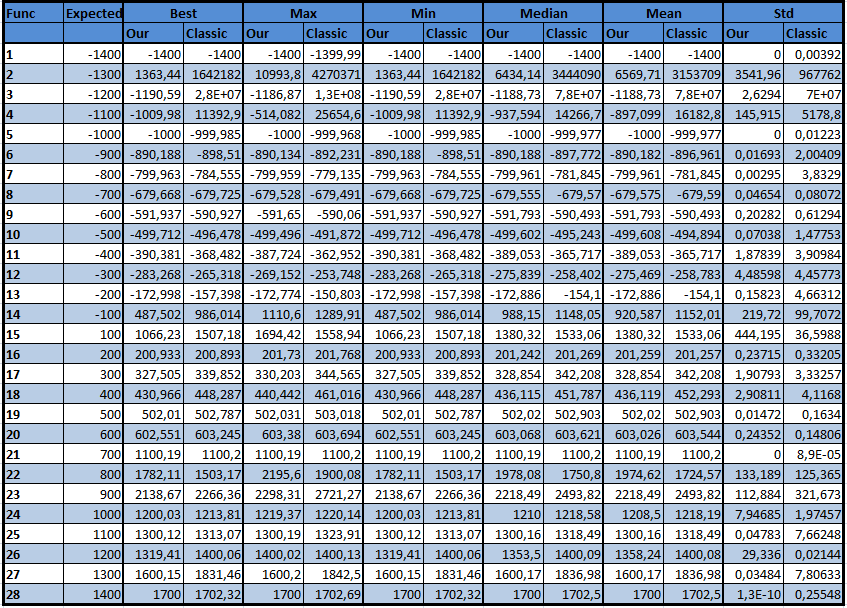
\includegraphics[width=\textwidth]{F75Cr75L10tab.png}
\caption{10-wymiarowa populacja. Wyniki dla parametrów: F = 0.75, Cr = 0.75}
\end{figure}

\begin{figure}[!h]
\centering
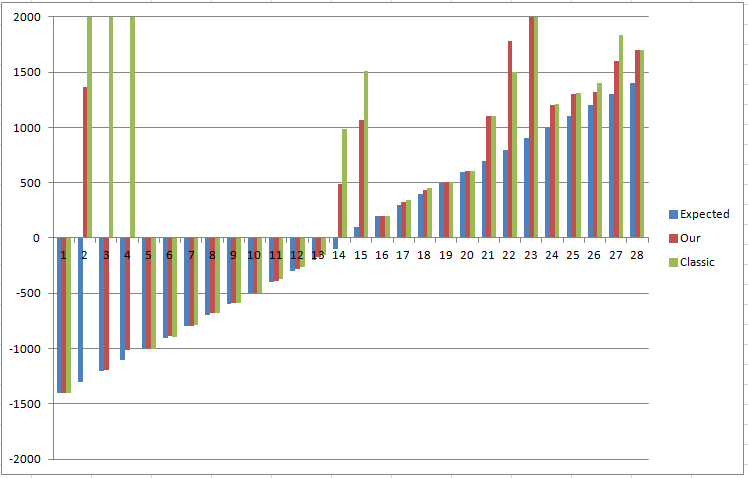
\includegraphics[width=\textwidth]{F75Cr75L10chart.png}
\caption{10-wymiarowa populacja. Wykres porównujący najlepsze rozwiązania dla naszego algorytmu oraz klasycznego. Parametry: F = 0.75, Cr = 0.75}
\end{figure}

\begin{figure}[!h]
\centering
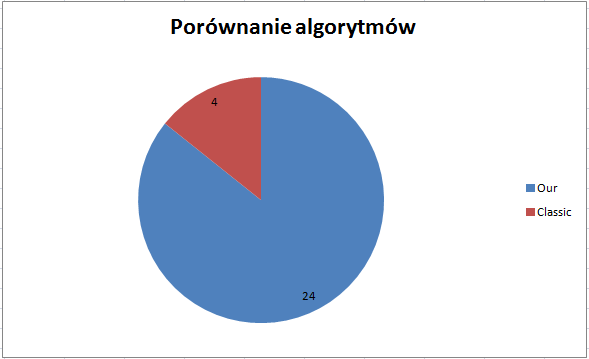
\includegraphics[width=\textwidth]{F75Cr75L10statystyka.png}
\caption{10-wymiarowa populacja. Parametry: F = 0.75, Cr = 0.75. Wykres porównujący liczbę lepiej znalezionych rozwiązań pomiędzy dwoma algorytmami.}
\end{figure}

\clearpage{}
\section{Wnioski}
Zarówno algorytm klasyczny, jak i z wyborem elementu średniego zwracaj porównywalne wyniki. Bardzo duże znaczenie na zwracane przez nie wyniki ma liczebność populacji początkowej oraz jej początkowe rozłożenie na przestrzeni rozwiązań. 

Najbardziej problematycznymi funkcjami dla obu algorytmów okazały się funkcje o indeksach 2, 3, 4. Często dla tych funkcji algorytmy dawały znacznie gorsze wyniki od oczekiwanego rozwiązania. Bardziej podatny na tego typu błędy okazał się algorytm klasyczny. 

Rozmiar wektora okazuje się mieć znaczenie na rozwiązanie. Dla wektorów 10-wymiarowych algorytmy częściej były podatne na pułapkę funkcji 2, 3, 4. Warto jednak zaznaczyć, że przyczyną tego może być fakt, że testowana liczebność populacji początkowej była równa dla obu wymiarów. 

Współczynniki $F$ i $c_r$ okazują się mieć znaczenie na działanie algorytmów. Wartości dające najlepsze rezultaty to $F=0.75$ i $c_r=0.75$. Jest to zauważalne dla algorytmu z wyborem elementu średniego dla obu wymiarów. Z kolei wartości przynoszące najgorsze rezultaty to $F=0.25$ i $c_r=0.25$. Można to wywnioskować na podstawie algorytmu z wyborem elementu średniego, który dla 10 wymiarów charakteryzuje się największą liczbą wartości znacznie odbiegających od oczekiwanych.

Podsumowując, oba algorytmy najlepiej działają dla mniejszej liczby wymiarów i dla współczynników $F=0.75$ i $c_r=0.75$. Dają dobre rezultaty, zbliżone bądź równe oczekiwanym wynikom. Częściej lepszy wynik zwracał algorytm z wyborem elementu średniego, co widać z wykresu \ref{rys:statystyka}.

\begin{figure}[!h]
\centering
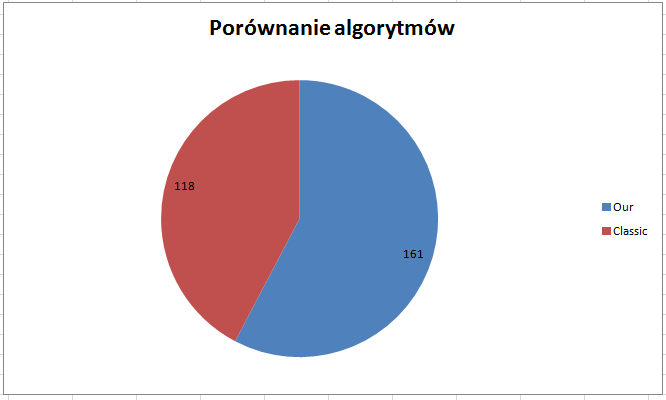
\includegraphics[width=\textwidth]{statystyka.png}
\caption{Ogólne porównanie skuteczności obu algorytmów.}
\label{rys:statystyka}
\end{figure}

\end{document}

